% Chapter5

\chapter{Implementation in Android Java and Metaio Tracking} \label{chapter:metaio}
\section{Android Platform}
We choose Android because it is the most popular mobile platform and we already had experience in developing apps for android. 

\subsection{Android Operation System}
Android is an operating system based on Linux with a Java programming interface.
\\


Android is currently primarily developed by Google.
\\


Android allows background processing, provides a rich user interface library, support
s 2-D and 3-D
graphics using the OpenGL libraries, access to the file system and provides an embedd
ed SQLite
database.\cite{androidDevTut}

\subsection{Android user interface components}
The most important user interface components ion android are: 

\begin{enumerate}
\item \textbf{Activity:} An Activity is the visible UI of an Android application. It contains so called \textit{widgets} for example buttons text-fields labels etc. to build a user interface. \cite{androidDevTut}

\item \textbf{Fragments:} Fragments
are components which run in the context of an
Activity. Fragments however make it easier to use build UIs for different sized devices.\cite{androidDevTut}


\item \textbf{Views and layout manager:} Views
are user interface widgets, e.g. buttons or text fields. They have attributes which can be used to configure their appearance
and behavior. (colour, size, onClick action, ..) \cite{androidDevTut}

\item \textbf{Layout XML:}
The user interface for Activities is typcally defined via XML files (layout files).\cite{androidDevTut}  But in this project we used HTML 5 and JQuery to make sure that the app could easily be ported to an other mobile platform just by re-writing the tracking logic to the specific system.

\item \textbf{Android Webview:} The WebView class is an extension of Android's View class that allows to display web pages as a part of the activity layout.\cite{androidWebView} As we already mentioned we choose this solution over plain Java-Android to achieve more platform independents.
\end{enumerate}   

\subsection{Develop an Android Application}
First of all the \textbf{Android SDK} is needed. The
Android Software Development Kit contains the necessary tools to create, compile and
package Android application.\cite{androidDevTut} 
\\


A compiled  
Android app is a \textbf{.APK} file which can be installed on a Android device. 
\\

The SDK also provides the \textbf{Android debug bridge}
(adb).A tool which allows to connect to an virtual or
real Android device.\cite{androidDevTut} We used this tool to test and debug our application.
 
\subsection{Android Manifest}
Every application must have an AndroidManifest.xml file in its root directory. The file describes essential information about the app. \cite{androidManifest}. For instance all activities, the app name, starting activity, size, etc. 
\\

It also contains al list of security permissions. We had to add the camera, internet, read\_owner\_data and get\_accounts permissions to implement all functions of our application. 


\begin{lstlisting}[language=xml, caption= 
extracts from our AndroidManifest]
<uses-permission android:name="android.permission.CAMERA" />
<uses-permission android:name="android.permission.INTERNET" />
 <uses-permission android:name="android.permission.READ_OWNER_DATA" />
<uses-permission android:name="android.permission.GET_ACCOUNTS" /> 
...
<!-- define an activity -->
<activity
	android:name=".TrackLogic"          
</activity>
\end{lstlisting}

\subsection{Creating an activity}
Every Android activity has to extend the \textbf{Activity} class and override the \textbf{onCreate} Method. onCreate gets executed when the activity is initialized.

\subsection{Android web-view}
We used the Activity sub-class \textbf{DroidGap} from \textbf{phonegap} to build activities. With this class it is easy to load webpages as view. 
\\



\begin{lstlisting}[language=java, caption= 
extracts from our source code]
public class MainMenue extends DroidGap {
	...
	public void onCreate(Bundle savedInstanceState)
	{
		..
		super.loadUrl("file:///android_asset/www/mainmenue.html", 1000);
		...
	}
}
\end{lstlisting}

The method \textbf{loadUrl} loads any web-page, doesn't matter if the URL is internal or external. It is also possible to pass an additional int time out parameter.   


\subsection{Java JavaScript Communication}
In the section above we mentioned that we used html pages to create the view of our application. Because of that we had to find a way to pass variables through, the in Java written activity, to the web-view. We accomplished that by using JavaScript. Again the activity has to extend the \textbf{DriodGap} class.
\\



First javascript must be enabled:
\begin{lstlisting}[language=java]
super.appView.getSettings().setJavaScriptEnabled(true);
\end{lstlisting}

Now its possible to pass variables to the html view:
\begin{lstlisting}[language=java]
int a=1;
super.loadUrl("javascript:{var myVariable=\""+a+"\";}");
\end{lstlisting}


\subsubsection{JavaScript Android Interface}
With such an interface it is possible to call activity methods form JavaScript. We needed them to react on button clicks from inside of the html view.  
\\

First we had to write a JavaScript function:
\begin{lstlisting}[language=html]
<script language="Javascript">
function trackClick() {
        MyTracking.performClick();
    }
</script>
..
<!-- set onCLick Action -->
<a href="#" onclick="trackClick();">Camera</a>
\end{lstlisting}





Then add a JavaScript interface to the activity:
\begin{lstlisting}[language=java]
super.addJavascriptInterface(new Object()
{
	public void performClick()
	{
		//react to button click
	}
},"MyTracking");
\end{lstlisting}

\section{Working with the Metaio SDK}
We used the Metaio SDK track and identify 3D or 2D Objects.


\subsection{Who is Metaio}
\begin{quotation}
"Metaio is the worldwide leader in Augmented Reality research and technology. Serving over 80,000 developers with over 1,000 apps for enterprise, marketing, retail, publishing and industrial cases, Metaio's AR software reaches over 30 Million consumers across the world." 
\begin{flushright}
(Metaio GmbH)
\end{flushright}
\end{quotation}

\subsection{Other Augmented Reality SDK's}
There are many other augmented reality technologies on the market: 
\begin{enumerate}
\item \textbf{Qualcomm Vuforia}: The Vuforia platform is mostly used for image recognition.

\item \textbf{Total Immersion D'Fusion}:
D'Fusion is the world's most widely-used commercial Augmented Reality solution. Unfortunately there are no free versions.

\item \textbf{Wikitude}: Wikitude is a powerful augmented reality sdk.However the cheapest SDK version costs 99\$.

\item \textbf{String}: String only recognises framed images. So this SDK was unusable for our application.  
\end{enumerate} \cite{augmentedRealitySDk}

In the End we choose Metaio SDK not only because our client recommended it but also because Metaio is a very powerful SDK. Unlike like most other technologies it has a free version and can track 3D objects. 
\\



Metaio also has a very big user community with a help-desk and many tutorials.   
 
\subsection{Metaio Toolbox}
The metaio Toolbox is an application used to create or edit 3D tracking maps of all textured objects in your surrounding.The created Maps than can be used in the Metaio SDK. We used the Toolbox-App to create 3D Maps of the cars our application is tracking.
\\ 

The Toolbox also allows you to play or edit AREL scenes. The AREL scene created in the metaio Creator can be directly played in the Toolbox. The geometries transformations can be edited in the Toolbox.
\\


Furthermore, the Toolbox also has camera calibration function that allows you to determine camera parameters of your device.  The Metaio Toolbox is a simple APP which is a available for Android and IOS. The APP can simply be downloaded and installed from Apple App-Store or Google Play.\cite{metaioToolBox}

Process of creating a Map:
\begin{enumerate}
\item Download and install Metaio Toolbox.
\item Open The App.
\item Tab on \textit{3D} Maps and than on \textit{new Map}. (It is also possible to edit existing map)
\item After that the camera opens and a Object can be tracked.
\end{enumerate}    
\begin{figure}[htbp]
\centering
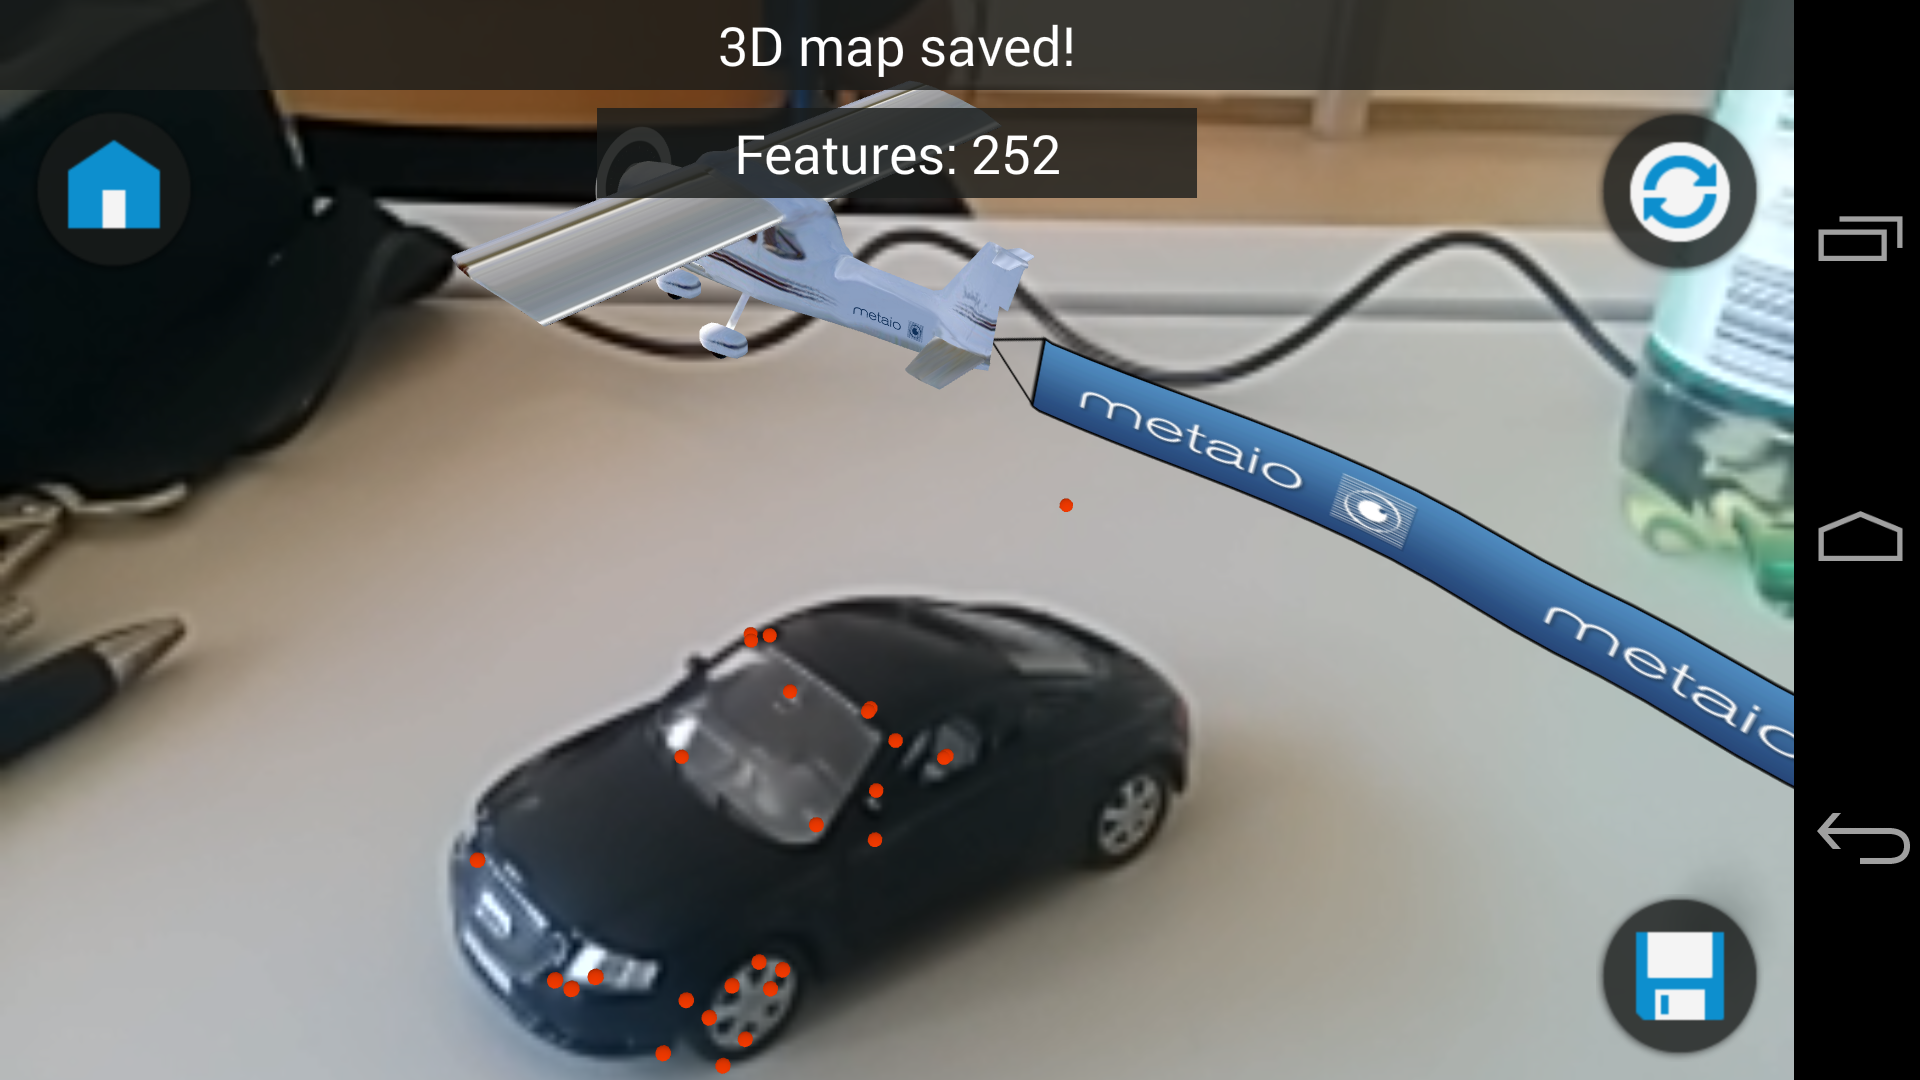
\includegraphics[width=\textwidth,height=\textheight,keepaspectratio]{graphics/tracking.png}
\caption{Metaio Tool Box}
\end{figure}
The red dots in the figure show the tracking points, the \textit{FEATURES} count shows how many tracking points have been placed. The more points the better can the object later be tracked by an application.

\subsection{AREL ( Augmented Reality Experience Language )} 
AREL ( Augmented Reality Experience Language ) is a JavaScript binding of the metaio SDK's API in combination with a static XML content definition

With Areal Scenes its possible to create a script with all tracking object and their behaviour, that scene than can be run by any metaio SDK. That's how you are able to create one platform independent Augmented Reality experience with AREL instead of using platform specific programming languages.
\begin{figure}[htbp]
\centering
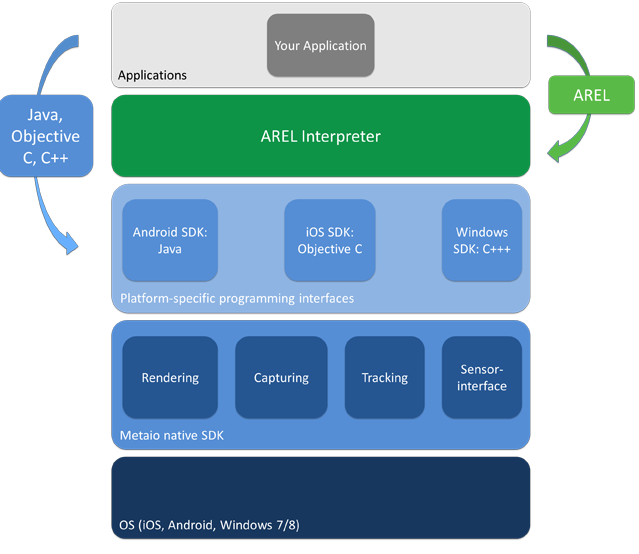
\includegraphics[width=\textwidth,height=\textheight,keepaspectratio]{graphics/arel.png}
\caption{AREL}
\end{figure}

AREL consists of the following parts:
\\

A XML Part which defines the content that should be loaded (3D-Models,Maps) and their size, position, transformation, etc. 
\\





The HTML 5 layer, this part provides graphical user interface and interacts using the JavaScript bridge with the metaio SDK. The AREL JavaScript bridge is a javascript library that allows to communicate with the Metaio SDK. All callbacks from the SDK are forwarded to the JavaScript Logic. \cite{metaioToolBox} 
\\

However AREL scenes where not use in the project because they only offered a limited size of Actions. For instance we needed to get the ID of the tracked object to determine which car had been recognized. It turned out that this is a much more difficult process in AREL so we wrote the whole logic in Java using the Metaio SDK.     

\subsection{Tracking XML}
The Tracking XML file is an XML file which can be created by the Metaio Creater or written by hand. It contains all of the tracking data. (3D Maps, etc. ..)
\begin{lstlisting}[language=xml, caption=Tracking XML example]
<?xml version='1.0' encoding='UTF-8'?>
<TrackingData>
	<Sensors>
		<Sensor subtype='ML3D' type='FeatureBasedSensorSource'>
			<SensorID>TrackingObject 1</SensorID>
			<Parameters>
				<featureorientationassignment>regular</featureorientationassignment>
			</Parameters>
			<SensorCOS>
				<SensorCosID>08921d8412c4de43d04eefc13c28ee3b</SensorCosID>
				<parameters>
					<numextensiblefeatures>0</numextensiblefeatures>
					<mintriangulationangle>6</mintriangulationangle>
					<map>08921d8412c4de43d04eefc13c28ee3b.f3b</map>
					<MinMatches>15</MinMatches>
					<DesiredMatchesRatioExtensible>0.35</DesiredMatchesRatioExtensible>
					<NumExtensibleFeatures>250</NumExtensibleFeatures>
				</parameters>
			</SensorCOS>	
	</Sensors>
</TrackingData>
\end{lstlisting}
All tracking Objects have to be added into the \textbf{Sensors} element. Every new object needs a \textbf{SensorCosID}, the name of the object. The \textbf{<Parameters>} element describes the 3D Map for the object. The map has to be in the same folder like the tracking xml. Other parameters are for instance the  \textbf{<MinMathes>} element, it describes how many points have to match so that the object gets recognised. Metaio has not really got a documentation for the Tracking XML therefore we choose to let the Metaio Creator create the xml file.


\subsection{Extracting the Tracking XML in Android}
In order to use xml file with the Metaio SDK, the tracking xml has to be placed in the \textbf{assets} folder of the android project.
\\


The files than have to be extracted by the \textit{AssetsManager} to make them accessible to the metaio SDK. This has to bee done in an Android \textit{AsyncTask}.
\\

The AsyncTask enables proper and easy use of the UI thread. This class allows to perform background operations and publish results on the UI thread. AsyncTasks should ideally be used for short operations (a few seconds at the most.) For threads that need to be running for long periods of time, it is recommended you use the various APIs provided by the java.util.concurrent pacakge such as \textit{Executor}, \textit{ThreadPoolExecutor} and \textit{FutureTask}.\cite{andoirdAsyncTask} 

\begin{lstlisting}[language=java, caption=Extracting Assets]
private class AssetsExtracter extends AsyncTask<Integer, Integer, Boolean>
{		
	@Override
	protected Boolean doInBackground(.. 
	{
		try 
		{
			// Extract all assets and overwrite existing files if debug build
			AssetsManager.extractAllAssets(...);
		} 
		catch (IOException e) 
		{
			//Error Messages
		}
			
		return true;
	}
		
	Override
	protected void onPostExecute(Boolean result) 
	{
		// Asset Path to the Tracking xml
		final String arelConfigFilePath = 
		  AssetsManager.getAssetPath("Tracking.xml");
		//Starting new Activity  
		Intent intent = new Intent(getApplicationContext(), 
		  TrackLogic.class);
		intent.putExtra(getPackageName()+".AREL_SCENE", 
		  arelConfigFilePath);
		startActivity(intent);

		finish();
	  }
}
\end{lstlisting}
The AsyncTask gets executed like this:

\begin{lstlisting}[language=java, caption=executing AsyncTask]
 AssetsExtracter asyncTask=new AssetsExtracter();
 //executing the task
 asyncTask.execute(0);
\end{lstlisting}





Android first runs the \textit{doInBackground} method, in this case the method extract all Assets using the Metaio 	AssetsManager: 	\textit{AssetsManager.extractAllAssets(...);}. After this method ends successfully the \textit{onPostExecute} method gets called.
\\


onPostExecute extracts the path to the tracking.xml and than starts the TrackingLogic class. This Activity is where the tracking happens.

\subsubsection{Loading the Tracking XML}
The TrackingLogic class in our project loads the tracking xml using the Metaio SDK:
\begin{lstlisting}[language=java, caption=executing AsyncTask]
String filepath = AssetsManager.getAssetPath("Tracking.xml");
...
// set the tracking configuration
 metaioSDK.setTrackingConfiguration(filepath); 
\end{lstlisting}

\section{Track Objects}
In order to run the camera and start the tracking process we wrote a new Activity which has to extend the Metaio \textbf{ARViewActivity}. Important methods provided by this class:
\begin{enumerate}
\item \textbf{loadContents():}This Method load the tracking xml.
\item \textbf{onTouch(View v, MotionEvent event):} By overwriting this method you can set what happens when the user touches the screen. 

\item \textbf{onGeometryTouched(final IGeometry geometry):} Metaio provides the possibility to draw 3D and 2D Models on the screen while tracking with the camera on, the method determines what happens when this geometry gets touched 

\item \textbf{onTrackingEvent(TrackingValuesVector trackingValues):} 
\\
One of the most important methods.onTrackingEvent describes what happens when an object gets tracked successfully. We overwrote this method to get the ID of the tracked Object. After the object hast been tracked the Main Menue activity with all specific car informations gets started.   
\end{enumerate} 
\begin{lstlisting}[language=java, caption= where the magic happens]
public void onTrackingEvent(TrackingValuesVector trackingValues)
{
 //Check through all maps 
 for (int i=0; i<trackingValues.size(); i++)
 {
  final TrackingValues v = trackingValues.get(i);
  if (v.isTrackingState())
  {
	Intent inte=new Intent(getApplicationContext(),MainMenue.class);
	//get id of tracked object
	inte.putExtra("id",""+v.getCoordinateSystemID());
	startActivity(inte);
	//close activity
	finish();
  }
				
 }
}
\end{lstlisting}
\section{Get Email Account from an Android device}
This product has  a small feature, it saves the email address from the smartphone and this email Address will be sent to the Navision Server. In this paragraph it describes how the project team implemented the feature in this Application.
Description \& Codesnippet:
This method will be invoked by the method getmail. This method will be explained in the next row. The getAccount() method  filters the Google Accounts . This happened through the Method getAccountsByType('com.google');.
Furthermore if the first object of the Account Array is bigger then the value of Account  it will be returned.

\begin{lstlisting}[language=java, caption= Accounts]
	private static Account getAccount(AccountManager accountManager) {
        Account[] accounts = accountManager.getAccountsByType("com.google");
        Account account;
        if (accounts.length > 0) {
            account = accounts[0];     
        } else {
            account = null;
        }
        return account;
    }

\end{lstlisting}

In this  Method it returns the Account object as String value. This happens through the Accountmanager and this method invokes the getAccount method. With the account Object it checks if it null if not then it returns the email address as String object.


\begin{lstlisting}[language=java, caption= Email]
static String getEmail(Context context) {
        AccountManager accountManager = AccountManager.get(context); 
        Account account = getAccount(accountManager);

        if (account == null) {
            return null;
        } else {
            return account.name;
        }
    }

\end{lstlisting}
The Email Address will be saved in a file , so the application  have to read the email address from the file. 